%%%%%%%%%%%%%%%%%%%%%%%%%%%%%%%%%%%%%%%%%
% Formal Text-Rich Title Page 
% LaTeX Template
% Version 1.0 (27/12/12)
%
% This template has been downloaded from:
% http://www.LaTeXTemplates.com
%
% Original author:
% Peter Wilson (herries.press@earthlink.net)
%
% License:
% CC BY-NC-SA 3.0 (http://creativecommons.org/licenses/by-nc-sa/3.0/)
% 
% Instructions for using this template:
% This title page compiles as is. If you wish to include this title page in 
% another document, you will need to copy everything before 
% \begin{document} into the preamble of your document. The title page is
% then included using \titleGP within your document.
%
%%%%%%%%%%%%%%%%%%%%%%%%%%%%%%%%%%%%%%%%%

%----------------------------------------------------------------------------------------
%	PACKAGES AND OTHER DOCUMENT CONFIGURATIONS
%----------------------------------------------------------------------------------------

\documentclass[a4paper]{article}
\usepackage[utf8]{inputenc}
\usepackage[spanish]{babel}
\usepackage{titlesec}
\usepackage{listings}
\usepackage{color}
\usepackage{pdfpages}
\usepackage{verbatim}
\titlelabel{\thetitle.\quad}
\lstset{
  language=C,                % choose the language of the code
  numbers=left,                   % where to put the line-numbers
  stepnumber=1,                   % the step between two line-numbers.        
  numbersep=5pt,                  % how far the line-numbers are from the code
  backgroundcolor=\color{white},  % choose the background color. You must add \usepackage{color}
  showspaces=false,               % show spaces adding particular underscores
  showstringspaces=false,         % underline spaces within strings
  showtabs=false,                 % show tabs within strings adding particular underscores
  tabsize=2,                      % sets default tabsize to 2 spaces
  captionpos=b,                   % sets the caption-position to bottom
  breaklines=true,                % sets automatic line breaking
  breakatwhitespace=true,         % sets if automatic breaks should only happen at whitespace
  title=\lstname,                 % show the filename of files included with \lstinputlisting;
}


%----------------------------------------------------------------------------------------
%	TITLE PAGE
%----------------------------------------------------------------------------------------

\newcommand*{\titleGP}{\begingroup % Create the command for including the title page in the document
\centering % Center all text
\vspace*{\baselineskip} % White space at the top of the page

\rule{\textwidth}{1.6pt}\vspace*{-\baselineskip}\vspace*{2pt} % Thick horizontal line
\rule{\textwidth}{0.4pt}\\[\baselineskip] % Thin horizontal line

{\LARGE \textbf{ORGANIZACIÓN DE COMPUTADORAS}\\[1\baselineskip]INFORME\\[0.2\baselineskip] TRABAJO PRÁCTICO 0}\\[0.2\baselineskip] % Title

\rule{\textwidth}{0.4pt}\vspace*{-\baselineskip}\vspace{3.2pt} % Thin horizontal line
\rule{\textwidth}{1.6pt}\\[\baselineskip] % Thick horizontal line

\vspace*{2\baselineskip} % Whitespace

\textbf{Alumnos} \\[\baselineskip]
{ 93198 - Peña, Maximiliano \\ maxipenia@gmail.com  \\[1\baselineskip]

 93665 - Poggio, Demian \\ demianpoggio@gmail.com  \\[1\baselineskip] 
 
 95505 - Iogha, Octavio \\ octaviomdq93@gmail.com \par} % Editor list

\vspace*{4\baselineskip} % Whitespace
	
% \textbf{Fecha de Entrega} \\[\baselineskip]
% { Martes 29 de Marzo }

\vspace*{4\baselineskip} % Whitespace

\textbf{Fecha de Vencimiento} \\[\baselineskip]
{ Martes 27 de Septiembre }

\endgroup}

%----------------------------------------------------------------------------------------
%	BLANK DOCUMENT
%----------------------------------------------------------------------------------------

\begin{document} 

\pagestyle{empty} % Removes page numbers

\titleGP % This command includes the title page

\newpage

\pagestyle{plain}

\section{Objetivos}
	El objetivo del trabajo práctico es familiarizarnos con las herramientas que necesitaremos para trabajar a lo largo de la cursada. Estas herramientas son:
	\begin{itemize}
	  \item Compilador GCC
	  \item Shell de Unix
	  \item Emulador GXEmul
	\end{itemize}

\section{Introducción Teórica}
  \label{sec:InfoTeo}
  Para poner en práctica estas herramientas, se debe implementar un programa en el lenguaje de programación C que permita, ingresando diversos parametros,
  generar imágenes en formato pgm correspondientes al conjunto de Julia y sus vecindades. Los parámetros para la generación de la imagen serán ingresados 
  al llamar al programa.
  A continuación se explican brevemente los conceptos necesarios para llevar a cabo esta tarea:

  \vspace{0.5cm}
	\subsection{Shell de Unix}
	  Un shell es un programa intérprete de comandos. Los comandos utilizados en el presente trabajo
	  son los siguientes:

	\subsection{Compilador GCC}
		GCC es un compilador gratuito, Open Source y multiplataforma que permite compilar código C. 
		El mismo es un compilador estándar, es decir, que respeta la norma ISOC99 o ANSI dependiendo de su versión, por lo cual se utilizan las 
		bibliotecas estándar para trabajar con el mismo. En esta asignatura el mismo es de gran utilidad dado que permite tener acceso  al código 
		\emph{assembly} equivalente a nuestro programa en C. A continuación se detallan brevemente algunos parámetros que podemos darle al GCC:
		\begin{itemize}
			\item \textbf{-Wall:} Activa todos los warnings.
			\item \textbf{-o file} Permite cambiar el nombre del archivo compilado generado.
			\item \textbf{-O0:} Desactiva las optimizaciones, lo cual resulta especialmente útil, porque genera código fácilmente entendible en 
			assembly en comparación al código C.
			\item \textbf{-O3:} Activa todas las optimizaciones, lo cual deseamos evitar, porque el código generado en assembly no se traduce de
			forma simple al código C correspondiente.
			\item \textbf{-g:} Genera código agregando información de debbugging.
			\item \textbf{-S:} Detiene el compilador luego de generar el código assembly.
			\item \textbf{-mrnames(solo para MIPS):} Indica al compilador que genera la salida utilizando nombre de registro en lugar de número de registro.
		\end{itemize}
		Para generar el archivo ``main.s'' con el código assembly se debe ejecutar el siguiente comando: 
		  \begin{verbatim}
			      gcc -std=c99 -S -mrnames -O0 -g tp0.c
		  \end{verbatim}
		Para compilar el código se debe ejecutar el siguiente comando:
		\begin{verbatim}
			      gcc -std=c99 -O0 -g tp0.c -o tp0 -lm
		 \end{verbatim}
		\vspace{0.5cm}
		
	\subsection{Emulador GXEmul}
		Es un emulador gratuito y Open Source de la arquitectuca de computadores MIPS. Tiene como ventajas que puede correr algunos sistemas operativos
		sin modificaciones como netBSD, su portabilidad y velocidad de emulación dado que realiza la traducción binaria en tiempo real. 
		\vspace{0.5cm}
		
		
\section{Diseño e implementación}
Para la implementación del programa se creó el archivo:
\begin{itemize}
	\item main.c: Contiene la implementación del software.
\end{itemize}

El programa utiliza los parámetros recibidos y comienza a realizar los calculos necesarios para generar la imagen del conjunto de Julia. Una vez que realiza los
calculos necesarios genera el documento pgm en donde guarda la imagen.

\subsection{Compilación}
Para compilar el programa basta con ejecutar 

\bigskip	
\begin{verbatim} gcc -std=c99 -O0 -g tp0.c -o <nombre salida> -lm \end{verbatim}


\subsection{Modo de Operación}
		La aplicación desarrollada recibe los parametros deseados y los utiliza para la generación de la imagen. Los mismos se describen a continuación:
		
		\begin{itemize}
			\item \begin{verbatim} tp0 -h  -V -c <a+bi>  -H <float>  -w <float>  -o <out file> \end{verbatim}
			\item \textbf{-V} Imprime la versión y finaliza.
			\item \textbf{-h} Imprime información y finaliza.
			\item \textbf{-c} Setea el centro de la imagen.
			\item \textbf{-H} Setea el alto del rectangulo. Valor por defecto=4.
			\item \textbf{-w} Setea el ancho del rectangulo. Valor por defecto=4.
			\item \textbf{-o} Setea el archivo de salida.
		\end{itemize}


		 \bigskip
Para ejecutarlo se debe hacer:

\bigskip
\texttt{\$ ./tp0 -o uno.pgm }

\bigskip
o

\bigskip
\texttt{./tp0 -C -1.125-0.21650635094611i -o dos.pgm}

	
\subsection{Ejecución de prueba}
     Primero, usamos la opcion -h para ver el mensaje de ayuda:
     \begin{verbatim}
Usage:
  tp0 -h  -V -c <a+bi> -C <a+bi> -H <float> -w <float> -o <out_file>
Options:
    -V	    Imprime la version y finaliza.
    -h	    Imprime esta informacion y finaliza.
    -c	    Setea el centro de la imagen.
    -H	    Setea el alto del rectangulo. Valor por defecto=4
    -w	    Setea el ancho del rectangulo. Valor por defecto=4
    -o	    Setea el archivo de salida
    -C	    Setea la constante del algoritmo. Valor por defecto= 0.285+0.01i
Examples:
  tp0 -c +0.282-0.01i -w 0.005 -H 0.005 -o dos.pgm
 	     \end{verbatim}
	     
Luego, hacemos una corrida de prueba con la linea:

\bigskip
\bigskip
\texttt{\$  ./tp0 -o uno.pgm}

\bigskip
Y el resultado de la ejecución fue:

\bigskip

\includegraphics[width=0.8\textwidth,natwidth=610,natheight=642]{uno.png}

\bigskip
Los resultados coinciden con los esperados, igual al ejemplo del enunciado.

\bigskip 
\bigskip 
Probamos con otro caso:

\bigskip
\texttt{\$  ./tp0 -C -1.125-0.21650635094611i -o dos.pgm}

\bigskip
Y el resultado de la ejecución fue:

\bigskip

\includegraphics[width=0.8\textwidth,natwidth=610,natheight=642]{dos.png}

\bigskip
Los resultados coinciden con los esperados, aunque invertidos respecto del ejemplo del enunciado.

\section{Corridas de prueba}

\subsection{Pruebas}

\subsubsection{Imagen 1x1}
\begin{verbatim}
./tp0 -c 0.01+0i -r 1x1 -o -
P2 
1 1 
255 
19 
\end{verbatim}
La salida es la esperada.

\subsubsection{Imagen 1x1 con punto que no pertenece al conjunto}
\begin{verbatim}
./tp0 -c 10+0i -r 1x1 -o -
P2 
1 1 
255 
0
\end{verbatim}
La salida es la esperada.

\section{Código fuente}

\lstinputlisting{tp0.c}

\bigskip

\section{Código MIPS}

\lstinputlisting{tp0.s}

\bigskip

%\lstinputlisting{main.s}

\section{Conclusión}
     En el presente trabajo se aprendió a utilizar las herramientas que utilizaremos en los próximos trabajos prácticos. 
     Se aprendió a utilizar el emulador GXEmul y compilar programas para arquitectura MIPS, tanto a forma binaria como assembly MIPS.

\section{Enunciado}

Adjundto a partir de la siguiente hoja.

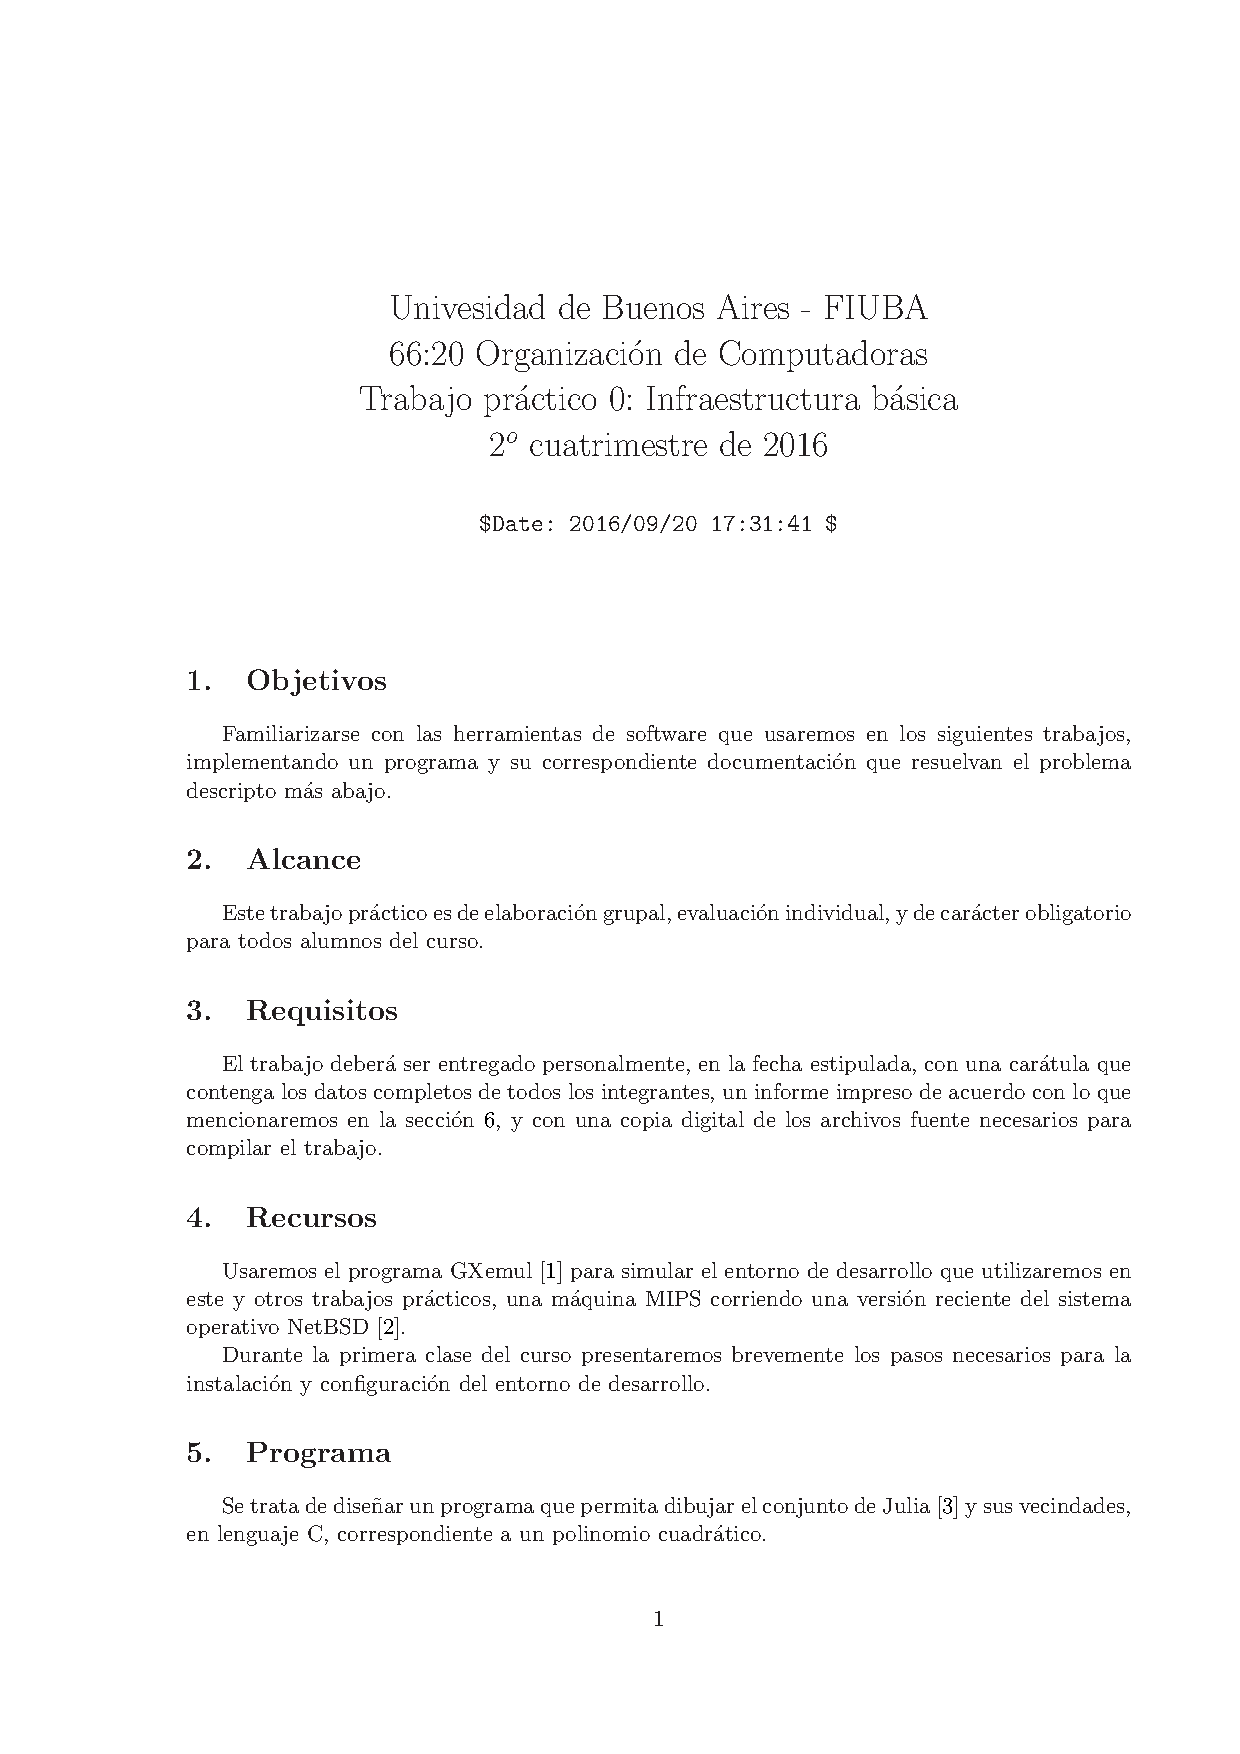
\includepdf[pages={-}]{enunciadoTp0.pdf}

\end{document}
